%Umfrage
\section{Nutzerstudie}
Im Rahmen der Bedürfnissermittlung wurde eine Nutzerstudie durchgeführt. Im Rahmen einer Onlineumfrage wurden 170 Personen (Stand: 27.05.2020) nach ihren Präfernezen und Hauptinteressen gefragt. Im folgenden werden die Ergebnisse vorgestellt.
Alle vorgestellten Ergebnisse beziehen sich auf den Stand der Studie am 27.05.2020\\

\subsection{Alterverteilung}
In der Umfrage wurde das Geburtsjahr der Teilnehmer abgefragt.
\\
\begin{figure}[h]
    \centering
    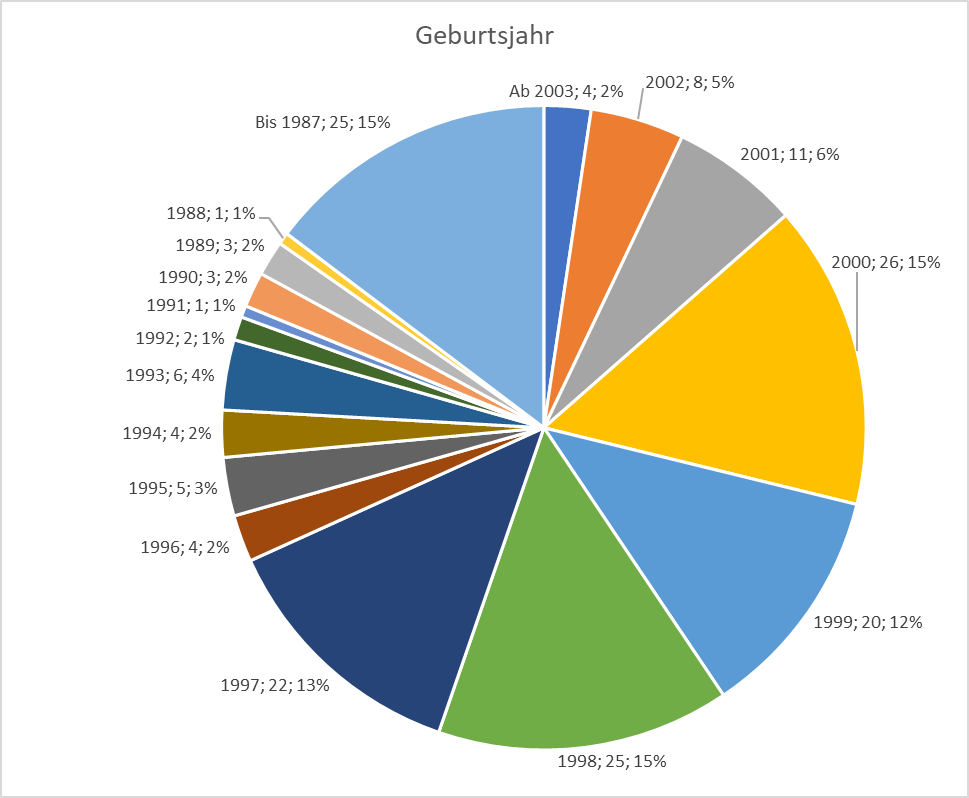
\includegraphics[scale=0.3]{media/diagram/geburtsjahr.png}
    \caption{Verteilung der Geburtsjahre der Befragten}
\end{figure}
\\
\subsection{Selbsteinschätzung von Wissen und Interesse am Thema Luftverschmutzung}
Für eine beurteilung des Interesses an den in \softwarename gezeigten Informationen wurde nach dem Interesse auf der Seite der nutzer gefragt.
Um abzuschätzen wie viel wissen bereits über Luftverschmutzung vorhanden ist wurde gefragt, wie die Nutzer ihr eigenes Wissen über Luftverschmutzung einschätzen.
\\
Bei beiden Einschätzungen wurde jeweils eine Zahl zwischen 1 und 5 abgefragt, wobei 1 sehr wichtig und 5 sehr unwichtig ist.
\\
\begin{figure}[h]
    \subfigure[Einschätzung zum eigenen Wissen über Luftverschmutzung]{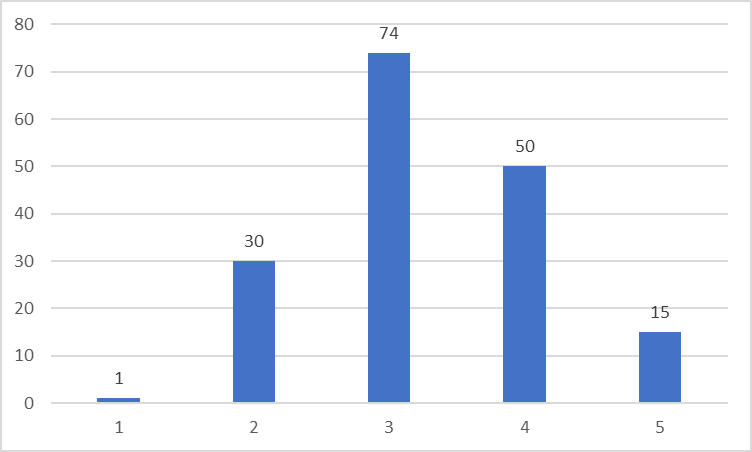
\includegraphics[width=0.49\textwidth]{media/diagram/eigenesWissen.png}}
    \subfigure[Einschätzung zur wichtigkeit von Informationen über Luftverschmutzung]{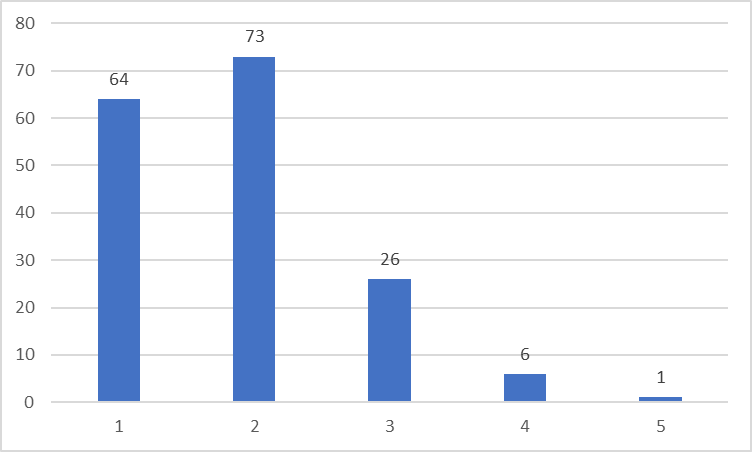
\includegraphics[width=0.49\textwidth]{media/diagram/WichtigkeitVonInfos.png}}
    \caption{Selbsteinschätzung der Nutzer}
\end{figure}
\\
Weiter wurden die Nutzer gefragt wie sie ihre Informationen zum Thema Luftverschmutzung erhalten. Die verbreitesten Informationsquellen sind hierbei
\begin{itemize} [noitemsep]
    \item Nachrichtensendungen und Berichterstattungen (circa 79\%)
    \item Informationen aus dem Internet (circa 78 \%)
    \item Gespräche mit anderen Personen (circa 26 \%)
\end{itemize}
Daraus ergibt sich, dass eine Webseite für die Vermittlung gut geeignet ist, da dieses Medium bereits weit verbreitet ist.

\subsection{Einschätzung zu Aufrufen der Webseite}

